\rhead{INTRODUCTION}
\lhead{}

\lettrine[lines=2,slope=0pt,nindent=4pt]{\textbf{L}}{a} Gestion de Configuration Logicielle (GCL) est une discipline de management de projet qui permet de d\'efinir,
d'identifier, de g\'erer et de contr\^oler les outils de configuration tout au long du cycle de d\'eveloppement d'un
logiciel. Cette gestion de configuration logicielle est r\'egie par la norme internationale ISO 10007:2017 \cite{normISO}. Le respect des normes internationales en terme de gestion de configuration est indispensable pour tout code, d'autant plus lorsque celui-ci est utilisé dans le cadre de la sûreté nucléaire comme l'est TrioCFD. Elle a pour objectif de r\'epondre \`a la question : " Quelqu'un a obtenu un r\'esultat. Comment le reproduire ? " Le plus souvent, il ne s'agit pas de reproduire \`a l'identique, mais de reproduire avec des modifications incr\'ementales. La question est donc de comparer des r\'esultats et d'analyser leurs diff\'erences.\smallskip\newline
La gestion de configuration du logiciel se concentre sur les aspects informatiques du logiciel et du syst\`eme qui le concerne. Ainsi, la GCL s'appuie sur la gestion de version pour pouvoir identifier avec fiabilité la version du logiciel utilis\'e, mais prend \'egalement en compte l'environnement mat\'eriel (machines h\^otes, \'equipements en interface) et syst\`eme (syst\`eme d'exploitation, type de r\'eseau,...) dans lequel celui-ci fonctionne.\newline
Elle s'attache \'egalement \`a tracer le suivi des \'evolutions (correctifs, \'evolutions) en regard des adaptations du produit. A ce titre, un outil de type \textit{syst\`eme de suivi de probl\`emes (issue tracking system)} est fortement recommand\'e dans le processus de gestion. Les adaptations qui en d\'ecoulent se font en veillant en maintenir \`a jour la matrice de conformit\'e qui garantit l'assurance fonctionnelle du produit.\smallskip\newline
En r\'esum\'e, g\'erer la configuration d'un logiciel consiste \`a g\'erer :
\begin{itemize}
	\item les diff\'erentes versions de ses composants (code, outils, donn\'ees de v\'erification/validation,...)
	\item sa documentation
	\item les anomalies et les r\'eponses apport\'ees \`a leur r\'esolution
	\item les demandes de modification ou d'\'evolution
	\item les environnements : espaces de d\'eveloppement, de v\'erification, de validation, de production
\end{itemize}

Cela consiste \'egalement \`a d\'efinir les r\`egles de passage d'un environnement \`a l'autre. Cette m\'ethodologie apporte au g\'enie logiciel les moyens de r\'ealiser un produit logiciel avec une qualit\'e et une ma\^itrise du processus de d\'eveloppement \'elev\'ees.\smallskip\newline
La Gestion de Configuration Logicielle permet de nombreux b\'en\'efices :
\begin{itemize}
	\item fournit une approche disciplinée et documentée pour d\'efinir, organiser et maintenir les \'el\'ements applicatifs,
	\item garantit l'int\'egrit\'e des applications,
	\item assure que les versions pr\'ec\'edentes de tout livrable contr\^ol\'e par configuration peuvent \^etre restaur\'ees et recr\'e\'ees,
	\item assure que tous les changements ne sont r\'ealis\'es que lorsque cela est requis et seulement par les personnes autoris\'ees.
\end{itemize}

Le Plan de Gestion de Configuration (PGC) permet, quant \`a lui, de fournir \`a l'\'equipe de d\'eveloppement et de validation du logiciel une m\'ethodologie de travail et une description de l'utilisation des  outils afin de r\'epondre aux exigences de fiabilit\'e qui leur sont demand\'ees. LE PGC est utilis\'e comme base pour r\'ealiser l'ensemble des activit\'es sur le code (maintenance, d\'eveloppement, correction, gestion de version, livraison,...).\smallskip\newline

L'objectif de ce Plan de Gestion de Configuration (PGC) de TrioCFD est donc de d\'efinir, pour les diff\'erents acteurs intervenants sur TrioCFD, les m\'ethodologies pour r\'esoudre les diff\'erentes actions qu'ils ont en charge, les outils \`a leur disposition ainsi que la documentation n\'ecessaire \`a la bonne utilisation du code.\smallskip\newline
Pour ce faire, nous commencerons par nous int\'eresser aux diff\'erents termes et acteurs de TrioCFD, puis aux outils de gestion. Les outils techniques sp\'ecifiques seront ensuite d\'ecrits ainsi que la m\'ethodologie de v\'erification et de validation. Nous finirons par la description de la conduite \'a tenir pour chacune des actions possibles sur le produit et les outils de communication autour de TrioCFD. Mais d\'ebutons, tout d'abord, par un petit historique de TrioCFD et une pr\'esentation g\'en\'erale de la structure du code.

\chapter{Un peu d'histoire}
\rhead{INTRODUCTION}
\lhead{Un peu d'histoire}

\lettrine[lines=2,slope=0pt,nindent=4pt]{\textbf{L}}{e} d\'eveloppement de TRIO\_U a d\'ebut\'e en 1994 au CEA de Grenoble avec l'ambition d'unifier TRIO VF, d\'evelopp\'e \`a Grenoble, Trio EF, d\'evelopp\'e \`a Saclay, et Genepi.\smallskip\newline
L'id\'ee initiale \'etait de cr\'eer un seul code unifi\'e (d'o\`u le \_U de TRIO\_U) code dans un langage plus r\'ecent \`a savoir le C++ puisque TRIO VF et Genepi \'etaient en Esope, TRIO EF en FORTRAN. Une premi\`ere maquette avait \'et\'e réalisée en se basant
sur le principe de cr\'eer une classe C++ par maille. Or, cette m\'ethodologie nécessitait des ressources machine beaucoup trop cons\'equentes pour les calculs fins. Un nouveau maquettage a \'et\'e alors réalisé avec une classe C++ par probl\`eme (Conduction, Hydraulique,...), par \'equation (\textit{e.g.} EDP), par op\'erateur (gradient, divergence, laplacien,...), par variable physique ($rho$, $mu$,..),... C'est cette seconde structure qui a \'et\'e finalement retenue et qui est, aujourd'hui encore, appliqu\'ee dans TRUST et ses Baltiks.\smallskip\newline
En ce qui concerne l'unification des codes, celle-ci ne s'est finalement pas faite et TRIO\_U a donc d\'ebut\'e uniquement avec TRIO VF et été d\'evelopp\'e sur Grenoble jusqu'\`a la migration du service de Thermohydraulique de Grenoble vers Saclay dans les ann\'ees 2010. Genepi est rest\'e un code ind\'ependant. Quant \`a TRIO EF, son d\'eveloppement n'a pas \'et\'e poursuivi.\smallskip\newline
Au fil des ann\'ees, les mod\`eles, fonctionnalit\'es et outils du code ont \'et\'e enrichis progressivement. L'historique de ces principales am\'eliorations sont pr\'ecis\'ees dans la frise chronologique \ref{figure:Histo-triou}.\smallskip\newline
En 2015, TRIO\_U v1.7.1 a \'et\'e scind\'e en deux parties : TrioCFD et TRUST. 
Cette s\'eparation entre TRUST et TrioCFD a \'et\'e faite de mani\`ere à ce que le code TRUST contienne toute la partie \texttt{noyau logiciel (kernel)} \'a savoir les op\'erateurs, les solveurs, la discr\'etisation, les outils de maillage et de post-traitement, les sch\'emas en espace et en temps et le parall\'elisme. TRUST est ainsi capable de r\'esoudre de mani\`ere autonome des probl\`emes laminaires monophasiques incompressibles ou quasi-compressibles en 2D ou 3D. TrioCFD regroupe, quant \`a lui, la partie \texttt{mod\`eles physiques pouss\'es pour la CFD} comme la turbulence
(LES et RANS), le diphasique (Front-tracking et Interface diffuse), les interactions fluide-structure (m\'ethode ALE),... Ces mod\`eles physiques sont rang\'es dans des modules distincts appel\'es \texttt{Baltik} faisant de TrioCFD un code modulaire.\newpage
\footnotesize
%\scriptsize
\begin{tikzpicture}
	\draw (8,0) -- (8,18.52) ;
	\draw (0,0) -- (0,0.01) ;
	\draw (7.8,18.52) -- (8.2,18.52) ;
	\draw (7.8,18.52) node[left]{$1994$} ;
	\draw[blue,thick,dashed] (8.0,18.52) -- (8.7,18.52) ;
	\draw[red] (8.8,18.52) node[right]{D\'ebut du projet Trio\_U} ;
	\draw[magenta,thick,dashed] (6.3,18.52) -- (7.0,18.52) ;
	\draw (6.2,18.52) node[left]{\textcolor{magenta}{Version en Unix}} ;
	\draw[decorate ,decoration={brace,amplitude=10pt,raise=0.5cm}] (8.35,18.32) -- (8.35,16.2) node[midway,right=1cm]{Maquettage};
	\draw (7.8,18.10) -- (8.0,18.10) ;
	\draw (7.8,17.68) -- (8.2,17.68) ;
	\draw (7.8,17.68) node[left]{$1995$} ;
	\draw (7.8,17.26) -- (8.0,17.26) ;
	\draw (7.8,16.84) -- (8.2,16.84) ;
	\draw (7.8,16.84) node[left]{$1996$} ;
	\draw[magenta,thick,dashed] (6.3,16.84) -- (7.0,16.84) ;
	\draw (6.2,16.84) node[left]{\textcolor{magenta}{Passage en gestion de configuration sous SCCS}} ;
	\draw (7.8,16.42) -- (8.0,16.42) ;
	\draw (7.8,16.00) -- (8.2,16.00) ;
	\draw (7.8,16.00) node[left]{$1997$} ;
	\draw[blue,thick,dashed] (8.0,16.00) -- (8.7,16.00) ;
	\draw (8.8,16.00) node[right]{\textcolor{blue}{v1.0} Discr\'etisation VDF seulement} ;
	\draw[green,thick,dashed] (6.3,16.00) -- (7.0,16.00) ;
	\draw[green] (6.2,16.00) node[left]{Mise en place des TNR} ;
	\draw (7.8,15.58) -- (8.0,15.58) ;
	\draw (7.8,15.16) -- (8.2,15.16) ;
	\draw (7.8,15.16) node[left]{$1998$} ;
	\draw[magenta,thick,dashed] (8.0,15.16) -- (8.7,15.16) ;
	\draw[magenta] (8.8,15.16) node[right]{Changement de gestionnaire de configuration : ClearCase} ;
	\draw[magenta,thick,dashed] (6.4,15.16) -- (7.0,15.16) ;
	\draw[magenta,thick,dashed] (6.4,15.37) -- (6.4,14.85) ;
	\draw[magenta,thick,dashed] (6.4,15.37) -- (6.3,15.37) ;
	\draw[magenta,thick,dashed] (6.4,14.85) -- (6.3,14.85) ;
	\draw[magenta] (6.2,15.37) node[left]{$1^{\`ere}$ Version Linux} ;
	\draw[magenta] (6.2,14.95) node[left]{$1^{\`ere}$ Maquette de parall\'elisme pour les machines CRAY} ;
	\draw (7.8,14.74) -- (8.0,14.74) ;
	\draw[blue,thick,dashed] (8.0,14.74) -- (8.7,14.74) ;
	\draw (8.8,14.74) node[right]{\textcolor{blue}{v1.1} Ajout de la discr\'etisation VEF} ;
	\draw (7.8,14.32) -- (8.2,14.32) ;
	\draw (7.8,14.32) node[left]{$1999$} ;
	\draw[cyan,thick,dashed] (8.0,14.32) -- (8.7,14.32) ;
	\draw[cyan] (8.8,14.32) node[right]{Visualisation des r\'esultats avec meshDV} ;
	\draw[cyan,thick,dashed] (6.3,14.32) -- (7.0,14.32) ;
	\draw[cyan] (6.2,14.32) node[left]{Interface avec Ansys ICEM CFD} ;
	\draw[cyan] (6.2,14.01) node[left]{(g\'en\'eration automatique du maillage pour TrioCFD)} ;
	\draw (7.8,13.90) -- (8.0,13.90) ;
	\draw (7.8,13.48) -- (8.2,13.48) ;
	\draw (7.8,13.48) node[left]{$2000$} ;
	\draw (7.8,13.06) -- (8.0,13.06) ;
	\draw[blue,thick,dashed] (8.0,13.06) -- (8.7,13.06) ;
	\draw[magenta] (8.8,13.06) node[right]{\textcolor{blue}{v1.2} $1^{\`ere}$ Version parall\`ele officielle} ;
	\draw (7.8,12.64) -- (8.2,12.64) ;
	\draw (7.8,12.64) node[left]{$2001$} ;
	\draw (7.8,12.22) -- (8.0,12.22) ;
	\draw[blue,thick,dashed] (8.0,12.22) -- (8.7,12.22) ;
	\draw (8.8,12.22) node[right]{\textcolor{blue}{v1.3} \textbf{Module} Rayonnement : mod\`eles de radiation} ;
	\draw (7.8,11.80) -- (8.2,11.80) ;
	\draw (7.8,11.80) node[left]{$2002$} ;
	\draw (7.8,11.38) -- (8.0,11.38) ;
	\draw[blue,thick,dashed] (8.0,11.27) -- (8.7,11.27) ;
	\draw (8.8,11.27) node[right]{\textcolor{blue}{v1.4} \textbf{Module} Turbulence : Ajout de nouveaux } ;
	\draw (10.0,10.87) node[right]{mod\`eles de turbulence pour la LES} ;
	\draw (7.8,10.96) -- (8.2,10.96) ;
	\draw (7.8,10.96) node[left]{$2003$} ;
	\draw[black,thick,dashed] (6.3,10.96) -- (7.0,10.96) ;
	\draw (6.2,10.96) node[left]{$1^{\`ere}$ version utilisable du Quasi-Compressible} ;
	\draw (7.8,10.54) -- (8.0,10.54) ;
	\draw (7.8,10.12) -- (8.2,10.12) ;
	\draw (7.8,10.12) node[left]{$2004$} ;
	\draw[cyan,thick,dashed] (8.0,10.12) -- (8.7,10.12) ;
	\draw[cyan] (8.8,10.12) node[right]{Remplacement de meshDV par VisIT} ;
	\draw[cyan,thick,dashed] (6.4,10.12) -- (7.0,10.12) ;
	\draw[cyan,thick,dashed] (6.4,10.33) -- (6.4,09.91) ;
	\draw[cyan,thick,dashed] (6.4,10.33) -- (6.3,10.33) ;
	\draw[cyan,thick,dashed] (6.4,09.91) -- (6.3,09.91) ;
	\draw[cyan] (6.2,10.33) node[left]{Utilisation du format MED} ;
	\draw[cyan] (6.2,09.91) node[left]{Interfa\c cage avec SALOME pour le maillage} ;
	\draw (7.8,09.70) -- (8.0,09.70) ;
	\draw (7.8,09.28) -- (8.2,09.28) ;
	\draw (7.8,09.28) node[left]{$2005$} ;
	\draw (7.8,08.86) -- (8.0,08.86) ;
	\draw (7.8,08.44) -- (8.2,08.44) ;
	\draw (7.8,08.44) node[left]{$2006$} ;
	\draw[blue,thick,dashed] (8.0,08.30) -- (8.7,08.30) ;
	\draw (8.8,08.30) node[right]{\textcolor{blue}{v1.5} \textbf{Module} Front-Tracking discontinu en VDF et VEF} ;
	\draw (7.8,08.02) -- (8.0,08.02) ;
	\draw (7.8,07.60) -- (8.2,07.60) ;
	\draw (7.8,07.60) node[left]{$2007$} ;
	\draw[magenta,thick,dashed] (6.3,07.60) -- (7.0,07.60) ;
	\draw[magenta] (6.2,07.60) node[left]{Interface de couplage ICoCo} ;
	\draw (7.8,07.18) -- (8.0,07.18) ;
	\draw[magenta,thick,dashed] (8.0,07.18) -- (8.7,07.18) ;
	\draw[magenta] (8.8,07.18) node[right]{Introduction de la notion de \texttt{BALTIK}} ;
	\draw (7.8,06.76) -- (8.2,06.76) ;
	\draw (7.8,06.76) node[left]{$2008$} ;
	\draw[magenta,thick,dashed] (8.0,06.76) -- (8.7,06.76) ;
	\draw[magenta] (8.8,06.76) node[right]{Introduction du solveur de syst\`emes lin\'eaires : PetSC} ;
	\draw[green,thick,dashed] (6.3,06.76) -- (7.0,06.76) ;
	\draw[green] (6.2,06.76) node[left]{Mise en place des fiches de validation automatiques} ;
	\draw (7.8,06.34) -- (8.0,06.34) ;
	\draw[magenta,thick,dashed] (6.3,06.21) -- (8.0,06.21) ;
	\draw (6.2,06.21) node[left]{\textcolor{blue}{v1.6} \textcolor{magenta}{Refonte de la structure des donn\'ees}} ;
	\draw (7.8,05.92) -- (8.2,05.92) ;
	\draw (7.8,05.92) node[left]{$2009$} ;
	\draw (7.8,05.50) -- (8.0,05.50) ;
	\draw (7.8,05.08) -- (8.2,05.08) ;
	\draw (7.8,05.08) node[left]{$2010$} ;
	\draw[magenta,thick,dashed] (8.0,05.08) -- (8.7,05.08) ;
	\draw[magenta] (8.8,5.08) node[right]{Autre m\'ethode de couplage avec MEDcoupling} ;
	\draw (7.8,04.66) -- (8.0,04.66) ;
	\draw (7.8,04.24) -- (8.2,04.24) ;
	\draw (7.8,04.24) node[left]{$2011$} ;
	\draw (7.8,03.82) -- (8.0,03.82) ;
	\draw (7.8,03.40) -- (8.2,03.40) ;
	\draw (7.8,03.40) node[left]{$2012$} ;
	\draw (7.8,02.98) -- (8.0,02.98) ;
	\draw (7.8,02.56) -- (8.2,02.56) ;
	\draw (7.8,02.56) node[left]{$2013$} ;
	\draw (7.8,02.14) -- (8.0,02.14) ;
	\draw[magenta,thick,dashed] (8.0,02.14) -- (8.7,02.14) ;
	\draw[magenta] (8.8,2.14) node[right]{Changement de gestionnaire de configuration : GIT} ;
	\draw (7.8,01.72) -- (8.2,01.72) ;
	\draw (7.8,01.72) node[left]{$2014$} ;
	\draw (7.8,01.30) -- (8.0,01.30) ;
	\draw (7.8,00.88) -- (8.2,00.88) ;
	\draw (7.8,00.88) node[left]{$2015$} ;
	\draw (7.8,00.46) -- (8.0,00.46) ;
	\draw[blue,thick,dashed] (8.0,00.46) -- (8.7,00.46) ;
	\draw[red] (8.8,00.46) node[right]{\textcolor{blue}{v1.7.1} S\'eparation de Trio\_U en TRUST \& TrioCFD} ;
	\draw[magenta,thick,dashed] (6.3,00.46) -- (8.0,00.46) ;
	\draw[magenta] (6.2,00.46) node[left]{Passage en OpenSource} ;
	\draw (7.8,00.04) -- (8.2,00.04) ;
	\draw (7.8,00.04) node[left]{$2016$} ;
\end{tikzpicture}\smallskip
\normalsize
\begin{center}\captionof{figure}{\label{figure:Histo-triou}Historique de Trio\_U. \small code couleur : \textcolor{blue}{version livr\'ee} -
\textcolor{cyan}{outils de visualistion et mailage} - \textcolor{green}{outils de documentation et validation} -
\textcolor{magenta}{outils informatiques et de couplage} - physique et num\'erique}\end{center}\smallskip
\normalsize

Malgr\`e cette scission, TrioCFD reste tr\`es proche de TRUST autant au niveau
des outils que de la gestion quotidienne. Les deux équipes de développement s'attachent \`a sortir les versions en 
m\^eme temps pour faciliter le processus de livraison. Chaque projet est g\'er\'e par 
une forge TULEAP propre (TRUST \& TrioCFD), il existe une forge d\'edi\'ee \`a l'administration des deux projets (TRUST admin CEA). Une bonne partie des documents utiles tout comme les formations utilisateurs et d\'eveloppeurs sont communes pour TrioCFD \& TRUST.\smallskip\newline

Depuis 2015 et la scission de TRUST et TrioCFD, les 2 codes ont continu\'e \`a \'evoluer, pour TRUST, sur les aspects outils, performances et optimisations et pour TrioCFD, sur les mod\`eles physiques et la documentation. Les \'evolutions de TRUST depuis 2015 ne sont pas d\'etaill\'es dans ce pr\'esent document puisque ce Plan de Gestion Logiciel concerne TrioCFD. Il est toutefois \`a noter qu'en 2020, deux am\'eliorations majeures ont \'et\'e apportées à TRUST :
\begin{itemize}
	\item possibilit\'e de lancement de calculs sur la partie GPU des processeurs
	\item passage du code en 64 bits
\end{itemize}
\vspace{1cm}
Pour TrioCFD, les \'evolutions majeures sont explicit\'ees sur la frise chronologique
\ref{figure:Histo-triocfd}.\smallskip

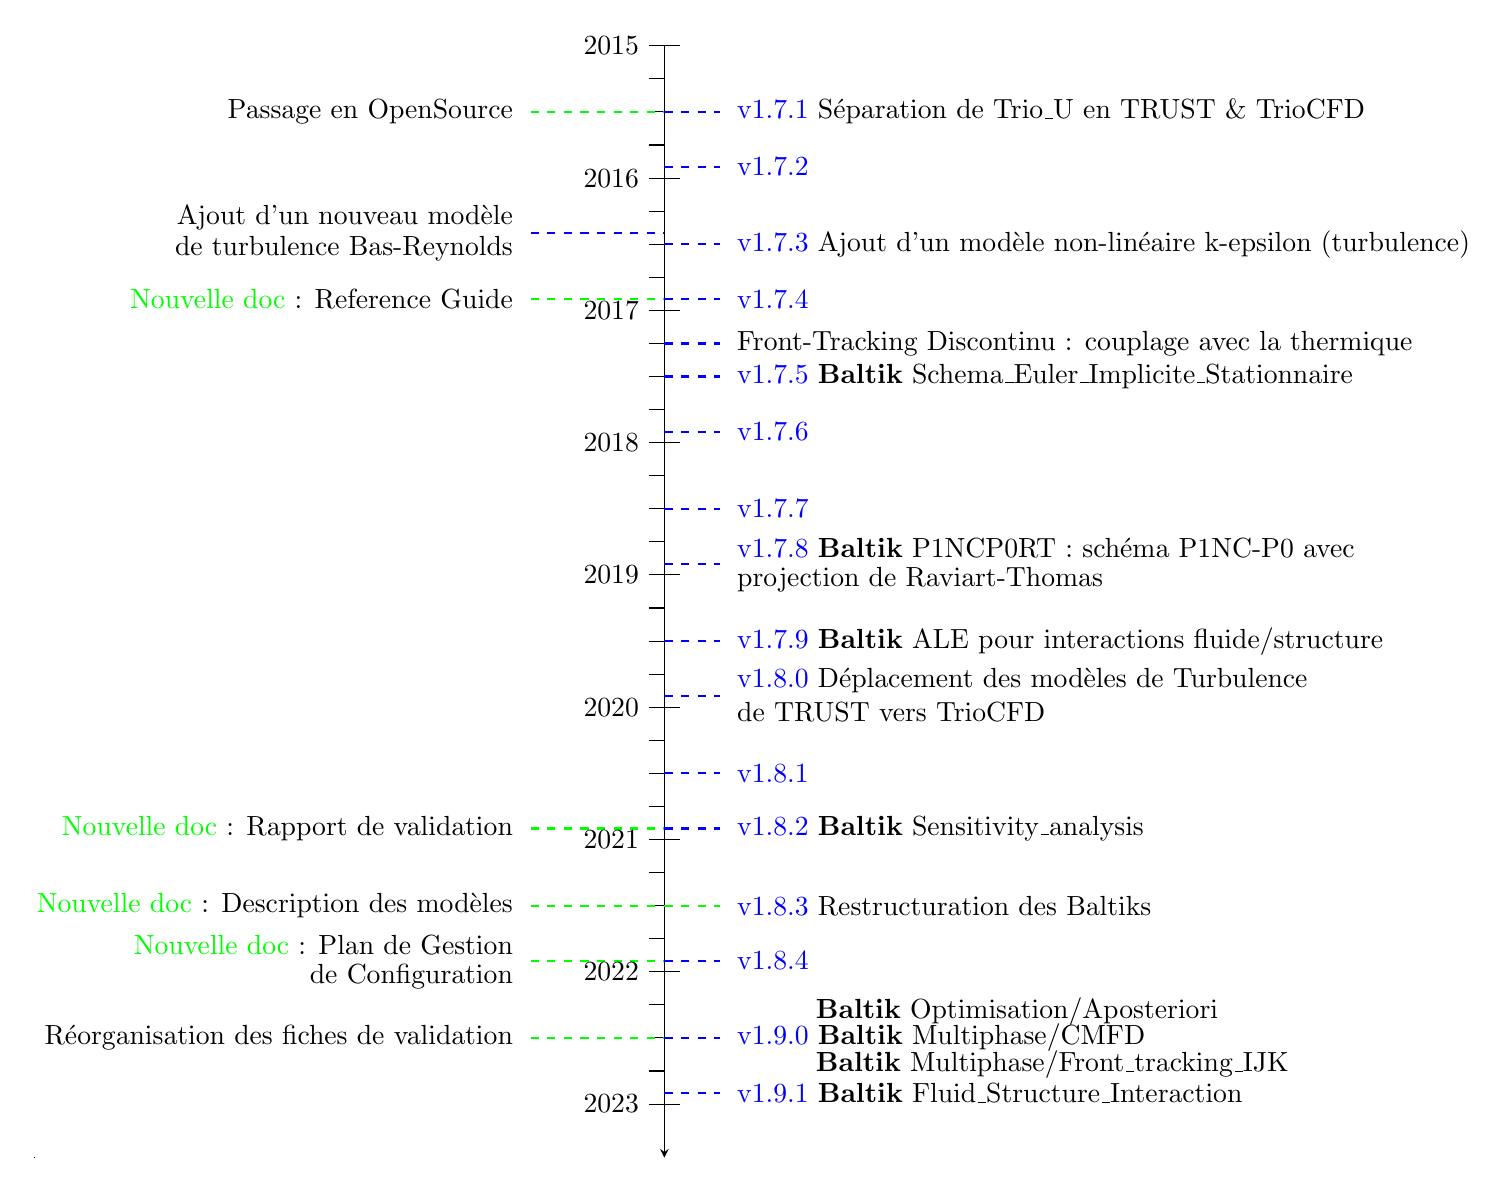
\begin{tikzpicture}
	\draw[<-,>=stealth] (8,0) -- (8,14.12) ;
	\draw (0,0) -- (0,0.01) ; 
	\draw (7.8,14.12) -- (8.2,14.12) ;
	\draw (7.8,14.12) node[left]{$2015$} ;
	\draw (7.8,13.70) -- (8.0,13.70) ;
	\draw (7.8,13.28) -- (8.0,13.28) ;
	\draw[blue,thick,dashed] (8.0,13.28) -- (8.7,13.28) ;
	\draw (8.8,13.28) node[right]{\textcolor{blue}{v1.7.1} S\'eparation de Trio\_U en TRUST \& TrioCFD} ;
	\draw[green,thick,dashed] (6.3,13.28) -- (8.0,13.28) ;
	\draw (6.2,13.28) node[left]{Passage en OpenSource} ;
	\draw (7.8,12.86) -- (8.0,12.86) ;
	\draw (7.8,12.44) -- (8.2,12.44) ;
	\draw[blue,thick,dashed] (8.0,12.58) -- (8.7,12.58) ;
	\draw (8.8,12.58) node[right]{\textcolor{blue}{v1.7.2}};
	\draw (7.8,12.44) node[left]{$2016$} ;
	\draw (7.8,12.02) -- (8.0,12.02) ;
	\draw (7.8,11.60) -- (8.0,11.60) ;
	\draw[blue,thick,dashed] (8.0,11.60) -- (8.7,11.60) ;
	\draw (8.8,11.60) node[right]{\textcolor{blue}{v1.7.3} Ajout d'un mod\`ele non-lin\'eaire k-epsilon (turbulence)} ;
	\draw[blue,thick,dashed] (6.3,11.74) -- (8.0,11.74) ;
	\draw (6.2,11.94) node[left]{Ajout d'un nouveau mod\`ele } ;
	\draw (6.2,11.54) node[left]{de turbulence Bas-Reynolds} ;
	\draw (7.8,11.18) -- (8.0,11.18) ;
	\draw[blue,thick,dashed] (8.0,10.90) -- (8.7,10.90) ;
	\draw (8.8,10.90) node[right]{\textcolor{blue}{v1.7.4}};
	\draw[green,thick,dashed] (6.3,10.90) -- (8.0,10.90) ;
	\draw (6.2,10.90) node[left]{\textcolor{green}{Nouvelle doc} : Reference Guide} ;
	\draw (7.8,10.76) -- (8.2,10.76) ;
	\draw (7.8,10.76) node[left]{$2017$} ;
	\draw (7.8,10.34) -- (8.0,10.34) ;
	\draw[blue,thick,dashed] (8.0,10.34) -- (8.7,10.34) ;
	\draw (8.8,10.34) node[right]{Front-Tracking Discontinu : couplage avec la thermique} ;
	\draw (7.8,09.92) -- (8.0,09.92) ;
	\draw[blue,thick,dashed] (8.0,09.92) -- (8.7,09.92) ;
	\draw (8.8,09.92) node[right]{\textcolor{blue}{v1.7.5} \textbf{Baltik} Schema\_Euler\_Implicite\_Stationnaire} ;
	\draw (7.8,09.50) -- (8.0,09.50) ;
	\draw[blue,thick,dashed] (8.0,09.22) -- (8.7,09.22) ;
	\draw (8.8,09.22) node[right]{\textcolor{blue}{v1.7.6}};
	\draw (7.8,09.08) -- (8.2,09.08) ;
	\draw (7.8,09.08) node[left]{$2018$} ;
	\draw (7.8,08.66) -- (8.0,08.66) ;
	\draw (7.8,08.24) -- (8.0,08.24) ;
	\draw[blue,thick,dashed] (8.0,08.24) -- (8.7,08.24) ;
	\draw (8.8,08.24) node[right]{\textcolor{blue}{v1.7.7}} ;
	\draw (7.8,07.82) -- (8.0,07.82) ;
	\draw[blue,thick,dashed] (8.0,07.54) -- (8.7,07.54) ;
	\draw (8.8,07.74) node[right]{\textcolor{blue}{v1.7.8} \textbf{Baltik} P1NCP0RT : sch\'ema P1NC-P0 avec} ;
	\draw (8.8,07.34) node[right]{projection de Raviart-Thomas} ;
	\draw (7.8,07.40) -- (8.2,07.40) ;
	\draw (7.8,07.40) node[left]{$2019$} ;
	\draw (7.8,06.98) -- (8.0,06.98) ;
	\draw (7.8,06.56) -- (8.0,06.56) ;
	\draw[blue,thick,dashed] (8.0,06.56) -- (8.7,06.56) ;
	\draw (8.8,06.56) node[right]{\textcolor{blue}{v1.7.9} \textbf{Baltik} ALE pour interactions fluide/structure} ;
	\draw (7.8,06.14) -- (8.0,06.14) ;
	\draw[blue,thick,dashed] (8.0,05.86) -- (8.7,05.86) ;
	\draw (8.8,06.06) node[right]{\textcolor{blue}{v1.8.0} D\'eplacement des mod\`eles de Turbulence } ;
	\draw (8.8,05.66) node[right]{de TRUST vers TrioCFD} ;
	\draw (7.8,05.72) -- (8.2,05.72) ;
	\draw (7.8,05.72) node[left]{$2020$} ;
	\draw (7.8,05.30) -- (8.0,05.30) ;
	\draw (7.8,04.88) -- (8.0,04.88) ;
	\draw[blue,thick,dashed] (8.0,04.88) -- (8.7,04.88) ;
	\draw (8.8,04.88) node[right]{\textcolor{blue}{v1.8.1}} ;
	\draw (7.8,04.46) -- (8.0,04.46) ;
	\draw (7.8,04.04) -- (8.2,04.04) ;
	\draw[blue,thick,dashed] (8.0,04.18) -- (8.7,04.18) ;
	\draw (8.8,04.18) node[right]{\textcolor{blue}{v1.8.2} \textbf{Baltik} Sensitivity\_analysis} ;
	\draw[green,thick,dashed] (6.3,04.18) -- (8.0,04.18) ;
	\draw (6.2,04.18) node[left]{\textcolor{green}{Nouvelle doc} : Rapport de validation} ;
	\draw (7.8,04.04) node[left]{$2021$} ;
	\draw (7.8,03.62) -- (8.0,03.62) ;
	\draw (7.8,03.20) -- (8.0,03.20) ;
	\draw[green,thick,dashed] (8.0,03.20) -- (8.7,03.20) ;
	\draw (8.8,03.20) node[right]{\textcolor{blue}{v1.8.3} Restructuration des Baltiks} ;
	\draw[green,thick,dashed] (6.3,03.20) -- (7.98,03.20) ;
	\draw (6.2,03.20) node[left]{\textcolor{green}{Nouvelle doc} : Description des mod\`eles} ;
	\draw (7.8,02.78) -- (8.0,02.78) ;
	\draw[green,thick,dashed] (6.3,02.50) -- (8.0,02.50) ;
	\draw (6.2,02.70) node[left]{\textcolor{green}{Nouvelle doc} : Plan de Gestion } ;
	\draw (6.2,02.30) node[left]{ de Configuration} ;
	\draw[blue,thick,dashed] (8.0,02.50) -- (8.7,02.50) ;
	\draw (8.8,02.50) node[right]{\textcolor{blue}{v1.8.4}};
	\draw (7.8,02.36) -- (8.2,02.36) ;
	\draw (7.8,02.36) node[left]{$2022$} ;
	\draw (7.8,01.94) -- (8.0,01.94) ;
	\draw (9.8,01.86) node[right]{\textbf{Baltik} Optimisation/Aposteriori};
	\draw (7.8,01.52) -- (8.0,01.52) ;
	\draw[blue,thick,dashed] (8.0,01.52) -- (8.7,01.52) ;
	\draw[green,thick,dashed] (6.3,01.52) -- (8.0,01.52) ;	
	\draw (6.2,01.52) node[left]{R\'eorganisation des fiches de validation} ;	
	\draw (8.8,01.52) node[right]{\textcolor{blue}{v1.9.0} \textbf{Baltik} Multiphase/CMFD};
	\draw (9.8,01.18) node[right]{\textbf{Baltik} Multiphase/Front\_tracking\_IJK};
	\draw (7.8,01.10) -- (8.0,01.10) ;
	\draw[blue,thick,dashed] (8.0,00.82) -- (8.7,00.82) ;
	\draw (8.8,00.82) node[right]{\textcolor{blue}{v1.9.1} \textbf{Baltik} Fluid\_Structure\_Interaction};
	\draw (7.8,00.68) -- (8.2,00.68) ;
	\draw (7.8,00.68) node[left]{$2023$} ;
%	\draw (7.8,01.84) -- (8.0,01.84) ;
%	\draw (7.8,01.42) -- (8.0,01.42) ;
%	\draw (7.8,01.00) -- (8.2,01.00) ;
%	\draw (7.8,01.00) node[left]{$2022$} ;
\end{tikzpicture}\smallskip
\begin{center}\captionof{figure}{\label{figure:Histo-triocfd}Historique de TrioCFD}\end{center}\smallskip
Il est \`a noter que m\^eme si TRUST supporte la partie "sch\'emas num\'eriques", lorsqu'un nouveau sch\'ema est amen\'e \`a \^etre d\'evelopp\'e pour des besoins TrioCFD, l'\'elaboration de ce nouveau sch\'ema est, dans un premier temps d\'evelopp\'e, v\'erif\'e et valid\'e dans TrioCFD avant d'\^etre revers\'e dans TRUST si d'autres Baltiks sous base TRUST (FLICA5, Genepi2,...) sont int\'eress\'es par ce sch\'ema.\newpage

Depuis la cr\'eation du projet, de nombreuses améliorations sur la parallélisme du produit ont permis d'augmenter, de manière très importante, les capacités de calcul. La plateforme TRUST/TrioCFD est maintenant en mesure d'effectuer des calculs haute performance (en anglais : High Performance Computing ou HPC). Les progrès récents (2020-2021) sur cet aspect viennent de 3 améliorations majeures :
\begin{itemize}
	\item \textbf{l'am\'elioration des processus d'entr\'ees/sorties :} le code utilise une base de	processeurs MPI pour \'ecrire certaines de ses donn\'ees de sortie. Cela signifie qu'il est n\'ecessaire d'avoir autant de processeurs MPI que de fichiers pour un seul calcul. Si cela est acceptable pour de petites simulations (jusqu'\`a 500-1000 n\oe{}uds MPI), cette m\'ethodologie n'est plus envisageable lorsque les calculs sont lanc\'es sur 10 000 n\oe{}uds MPI ou plus. Gr\^ace au support du format HDF5, le processus a 	\'et\'e rationnalis\'e. La structure des donn\'ees reste similaire (une donn\'ee par processeur) mais un fichier physique donn\'e est d\'esormais remplac\'e par un ensemble de donn\'ees correspondant, dans un seul 	fichier HDF5. Cette strat\'egie a \'et\'e mise en place dans les cas/situations les plus gourmands en terme de ressources machine (fichiers de v\'erification, fichiers de sauvegarde/reprise, stockage des informations de 	division de domaine,...) permettant ainsi une r\'eduction drastique de nombre d'i-nodes utilis\'es sur le système de fichiers du cluster.
	\item \textbf{le portage du code sur des identifiants 64 bits :} pour les tailles de maillage n\'ecessaires dans une simulation massive, le format 32 bits s'est av\'er\'e trop restrictif. En effet, les diverses entit\'es du maillage (sommets, faces, volumes) d'un maillage de 2 millards d'\'el\'ements ne peuvent pas \^etre index\'ees en utilisant seulement 4 octets (32 bits). Le noyau du code C++ ainsi que divers outils 	accompagnant la plateforme (notamment les plugins de visualisation pour le logiciel VisIt) ont \'et\'e port\'es sur une indexation en 64 bits.
	\item \textbf{l'optimisation de la m\'emoire :} la plateforme TRUST/TrioCFD s'appuie fortement sur la biblioth\`eque PETSc (manipulation des vecteurs et matrices denses et creuses et r\'esolution de syst\`emes lin\'eaires) et certaines des matrices du calcul, notamment la matrice jacobienne utilis\'ee dans les sch\'emas num\'eriques implicites, n'\'etaient, jusqu'\`a pr\'esent, pas remplies de fa\c con optimale. Des optimisations ont \'et\'e faites dans ce sens.
\end{itemize}

Gr\^ace \`a ces am\'eliorations sur la parall\'elisation et les performances, TRUST/TrioCFD est d\'esormais capable de r\'esoudre des simulations extrêmement fines en utilisant la parall\'elisation massive. Le tableau \ref{tab:perfo} retrace les \'evolutions en terme de puissance de calcul de la plateforme.
\begin{table}[H]
\begin{centering}
\footnotesize
\begin{tabular}{Sc Sc Sc}
\hline\hline
\rowcolor{lightgray}\textbf{Ann\'ee} & \textbf{nombre d'\'el\'ements du maillage}  & \textbf{nombre de c\oe{}urs} \tabularnewline
\hline
1999 & 10 millions &  \tabularnewline\hline
2010 & 500 millions & 10 000\tabularnewline\hline
2020 & 1 milliard & 17 000 \tabularnewline\hline
2021 & 2 milliards & 50 000\tabularnewline
\hline\hline
\end{tabular}
\normalsize
\par\end{centering}
\caption{\label{tab:perfo}Evolution des performances de calcul de la plateforme TRUST/TrioCFD}
\end{table}


\chapter{Pr\'esentation g\'en\'erale et cartographie}
\rhead{INTRODUCTION}
\lhead{Pr\'esentation et cartographie}

\lettrine[lines=2,slope=0pt,nindent=4pt]{\textbf{D}}{epuis} la s\'eparation de TRUST et TrioCFD, TrioCFD est devenu un \texttt{Baltik} (\textbf{B}uild an \textbf{A}pplication \textbf{L}inked to \textbf{T}r\textbf{i}o\_U \textbf{K}ernel) de TRUST. Cela implique que TrioCFD h\'erite de tous les outils de TRUST \`a savoir :
\begin{itemize}[label=$\Rightarrow$, font=\LARGE]
  \item \textbf{La discr\'etisation :}
  \begin{itemize}
    \item Finite Volume Difference (VDF) ou Volumes Finis
    \item Finite Volume Element (VEF) ou El\'ements Finis
    \item PolyMach
  \end{itemize}
  \item \textbf{Conditions aux limites :} pour les parois et le fluide
  \item \textbf{Sch\'emas en temps :}
  \begin{itemize}
    \item explicite : Euler, Runge-Kutta, Adams-Bashforth, Crank-Nicholson
    \item semi-implicite
    \item implicite : Euler, Adams-Moulton, backward differentiation
  \end{itemize}
  \item \textbf{Sch\'emas en espace pour la convection :}
  \begin{itemize}
    \item jusqu'au $4^{\`eme}$ ordre
    \item upwind, centered stabilized, MUSCL, QUICK, ...
  \end{itemize}
  \item \textbf{Les outils de de g\'en\'eration de maillage :}
  \begin{itemize}
    \item l'outil interne \`a TRUST pour les cas les plus simples
    \item SALOME \cite{Salome}
    \item Gmesh \cite{Gmesh}
  \end{itemize}
  \item \textbf{Post-traitement :}
  \begin{itemize}
    \item sur les variables principales
    \item sur les propriétés physiques
    \item sur (quasiment) ce qu'on veut via des sondes définies dans le jdd
    \item visualisation : SALOME, VisIT, GnuPlot
  \end{itemize}
  \item \textbf{Cas tests automatisés :}
  \begin{itemize}
    \item fiches de validation (.prm)
    \item g\'en\'eration d'un rapport pdf par prm
    \item comparaison pixel \`a pixel des pdf pour le processus de validation
  \end{itemize}
  \item \textbf{Suivi de l'impact des autres BALTIKs sur TrioCFD}
  \item \textbf{HPC (High Performance Computing) :}
  \begin{itemize}
    \item parallélisme massif (MPI)
    \item pr\'esent sur les calculateurs CEA (cluster CURIE : 2 petaFLOPS - cluster AIRAIN : 420 teraFLOPS)
  \end{itemize}
\end{itemize}\smallskip

Tous ces outils étant hérités de TRUST, leur gestion est du ressort de l'équipe TRUST. Par conséquent, leur processus ne sera pas décrit dans ce présent PGC. Toutefois, une description de certains de ces outils sera faite dans les sections suivantes.\\
TrioCFD est en langage C++ pour la partie source du code tandis que les procédures sont en Python ou en bash. Le code source est constitué d'environ 1 500 classes et 513 636 lignes de code (fichiers .cpp et .h). La mod\'elisation d'un applicatif considéré est définie dans un Jeu De Données (.data) et toutes les ex\'ecutions (compilation du code, lancement du jeu de données,...) se font en ligne de commande. \smallskip\\

TrioCFD est lui-même composé de plusieurs Baltiks et sous-Baltiks ayant tous un domaine de compétence spécifique. Ils sont \`a l'heure actuelle au nombre de 10 et 2 d'entre eux contiennent eux-même 2 sous-Baltiks. Le tableau \ref{tab:carto-baltiks} dresse la liste de ces Baltiks et sous-Baltiks, leur domaine de compétence ainsi que leur dépendance interne.

\begin{table}[H]
\begin{centering}
\footnotesize
\begin{tabular}{Sc Sc Sc}
\hline\hline
\rowcolor{lightgray}\textbf{Baltik} & \textbf{Description}  & \textbf{D\'ependances} \tabularnewline
\hline

\textbf{Critere\_Entrainement\_Gaz} & Crit\`ere num\'erique bas\'e sur la voriticit\'e & Turbulence \tabularnewline
& pour pr\'edire l'aparition d'un vortex & Turbulence \tabularnewline\hline
 & M\'ethode Arbitrary Langrangian-Eulerian  & Turbulence \tabularnewline
\textbf{Fluid\_Structure\_Interaction} & pour les interactions fluide-structure & \tabularnewline
  & mod\`ele vibratoire de poutre & \tabularnewline\hline
\textbf{Multiphase} & & \tabularnewline
$\hookrightarrow$ CMFD & Computational Multiphase Fluid Dynamics  & SO \tabularnewline
$\hookrightarrow$ Front\_tracking\_IJK & Int\'egration de TrioIJK dans TrioCFD  & Turbulence \& FTD \tabularnewline
$\hookrightarrow$ Front\_tracking\_discontinu & Suivi d'interface avec la méthode de Front-Tracking & Turbulence \tabularnewline
$\hookrightarrow$ Phase\_field & Écoulements diphasiques incompressibles de & SO \tabularnewline
& fluides non miscibles & \tabularnewline\hline
\textbf{P1NCP0RT} & Approximation P1/P0 non conforme avec les &  \tabularnewline
& éléments de Raviart-Thomas & SO \tabularnewline\hline
\textbf{Rayonnement} & Rayonnement thermique & \tabularnewline
$\hookrightarrow$ Rayonnement\_milieu\_transparent & dans différents & Turbulence \tabularnewline
$\hookrightarrow$ Rayonnement\_semi\_transp & milieux & Turbulence \tabularnewline\hline
\textbf{Schema\_Euler\_Implicite\_Stationnaire} &  & Turbulence \tabularnewline\hline
& Quantification des changements dans la solution d'un & \tabularnewline
\textbf{Sensitivity\_analysis} &  système d'EDP (ici Navier-Stokes) dus aux variations & SO \tabularnewline
& des paramètres d'entrée & \tabularnewline\hline
& Baltik principal de TrioCFD dont quasiment & \tabularnewline
\textbf{Turbulence} & tous les autres Baltiks dépendent. Il contient l'ensemble & SO \tabularnewline
& des modèles de turbulence (Bas-Reynolds, k-epsilon, & \tabularnewline
& lois de parois,...) quelle que soit la discrétisation considérée & \tabularnewline\hline
& Baltik contenant les fiches de validation pour & \tabularnewline
\textbf{validation} & les tests à effets intégraux. Les fiches de validation & Turbulence \tabularnewline
& des tests à effets séparés sont présents dans le répertoire & \tabularnewline
& \texttt{/share} du Baltik concerné &  \tabularnewline\hline
\textbf{Zoom} & & Turbulence \tabularnewline
\hline\hline
\end{tabular}
\normalsize
\par\end{centering}
\caption{\label{tab:carto-baltiks}Cartographie des BALTIKS et sous-BALTIKS de TrioCFD}
\end{table}

Ces différents Baltiks permettent de couvrir les domaines de modélisation physique suivants :
\begin{itemize}[label=$\Rightarrow$, font=\LARGE]
  \item Hydraulique avec ou sans turbulence
  \item Thermohydraulique avec ou sans turbulence
  \item Quasi-compressible
  \item Écoulements diphasiques
  \begin{itemize}
    \item Front-Tracking
    \item Interface diffuse incompressible
    \item Modèle Homogène Équilibré (HEM) pr\'esent dans le Baltik CMFD
  \end{itemize}
  \item Interactions fluide/structure par la méthode ALE
  \item Chimie
\end{itemize}

Les outils seront décrits dans la troisième partie de ce document mais avant cela, intéressons nous aux différents termes spécifiques qui seront utilisés par la suite.
